\documentclass[]{report}
\renewcommand\thesection{\arabic{section}}%for page numbering in arabics
\usepackage{graphicx,tabularx}%for figures and tables
\usepackage[utf8]{inputenc} %allows special characters such as ä, ö, ỳ
\usepackage[english]{babel}  %set the language to English
\usepackage[margin=1.5in]{geometry} %change page margins 
\usepackage{sectsty}%section headers
\allsectionsfont{\sffamily\large}
\subsectionfont{\sffamily\normalsize}
\linespread{1.2}% line distance
\usepackage{lipsum}% http://ctan.org/pkg/lipsum
\usepackage{caption}%use for captions on tables
%use this exact command. The style and bibliographystyle has to be authoryear (Havard). The sorting is nyt: name, year, title so that the bibliography is sorted alphabetically. firstinits=true shortens the names: Albert Einstein -> A. Einstein
\usepackage[backend=bibtex,style=authoryear,bibstyle=authoryear,sorting=nyt,firstinits=true]{biblatex}
\setlength\parindent{0pt}%include this so that your paragraphs don't indent automatically
\addbibresource{library.bib} %this attaches your bib-file, your bibliography (must be in the same folder)
\usepackage[compact]{titlesec}%include title formatting package
\usepackage{enumitem}
\setlist{nolistsep}

% Title Page
\title{What role does latency play in the wide-spread adaptation of cloud gaming?}
\author{Jamie Meyer and Glenn Verstraelen}
\date{December 14th 2021 \\Module: SEAR \\Venlo, Limburg, Netherlands}


\begin{document}
\maketitle

\begin{abstract}
This is the abstract.
\pagenumbering{roman}
\end{abstract}

\tableofcontents
\setcounter{page}{3}
%\listoffigures %UNCOMMENT IF YOU HAVE FIGURES
%\listoftables %UNCOMMENT IF YOU HAVE TABLES
\pagebreak
\pagenumbering{arabic}	
	
\section{Introduction}

\subsection{What is a cloud gaming service?}
Cloud gaming is a method of playing video games using a remote servers which essentially run the video game and stream the game play to your local device.
This local device can be any device which the cloud gaming service supports,
this can differ from provider to provider but most support all relevant platforms: mobile, desktop, console and the web.\\\\ 
The amount of freedom you get with a specific cloud gaming service also differs from provider to provider some services only allow you to play games that are available in their catalog, while others pretty much give you remote access to a full on high end gaming computer where you can play and do anything on. Some providers also give additional benefits such as free games and a free controller whenever you sign up for their service.\\\\
Cloud gaming does require the user to have a good and stable internet connection for a good experience but since internet speeds are getting faster and more accessible to larger groups of people cloud gaming will become a more competitive option for people to choose from, especially with current shortages in computer hardware and increased prices in video game consoles.  

\subsection{How do we define latency in this context?}
Latency in this research is defined as the time it takes for the client to pass a data packet from their place to another. Latency can be determined by many possible factors, such as: Internet connection speed, the distance between the client and host, internet traffic, servers that are overloaded, the connection between the client's console and router, router settings not optimized for gaming, low memory space or old system hardware.\\\\
Whether the client is using a wired or a wireless network, both types share latency, but the difference is noticeable. While a normal wired network doesn't quite travel at the speed of light, the latency is almost imperceptible to humans, being a 12-34 ms delay (fiber or cable internet). When a wireless network is being used by the client, the latency depends on the type of GHz that is being used, which in this case is 2.4 and 5 GHz. Where 2.4 GHz can be used in a large covered area having wall penetration, the low data rate is one of the key points where latency can occur. And while 5 GHz has a smaller covered area with no wall penetration, it uses orthogonal frequency division multiplexing (OFDM) which creates a high data rate that keeps latency lower than what a 2.4 GHz network type can create.\\\\
Latency can be an annoyance, to some extend. For people who don't normally play video games or online games and use their network (mostly) for social media, Internet searches, or messaging services, it's usually not a big problem. But for the people who do use their network to play online video games, it is disruptive. In an online video game, it is convenient (or even mandatory) for the person to play without internet interference, to perform the right actions at the right time. But when the latency in their game is high, the player is often stuck on the frame where he/she was a few seconds ago and has (almost) no flexibility in their game. This is only for games that require an internet connection, where games that doesn't need one can run smoothly without latency issues (depending on your hardware).\\\\
So what about cloud gaming, a game that doesn't require an internet connection to play just runs without problems right? Unfortunately the problems are exactly the same as with an online game that is not attached to cloud gaming. Even if you play an offline game via cloud gaming, it still means that you can experience input latency. For example, where the player presses a button that is seen as a jump function, it might take more than 1-2 seconds for the input to be received by the host and send back to the player, which can make the game play very difficult.
\subsection{Popular cloud gaming services}
While cloud gaming would not be the first option for most video game players, mainly because most already have a home console or gaming computer in their homes or maybe because the internet connection is not always good, some companies have managed to make cloud gaming usable for the customer. Cloud gaming services such as Shadow, GeForce Now and Google Stadia have been well received by customers in the year 2021.\\\\
\textbf{Shadow}\\
\citetitle{shadow} is a cloud gaming service that is available for Windows, Mac, smartphone, tablet and for the television. The service requires a strong internet connection with 15 Mbps at the minimum for the best performance.\\\\
Shadow gives the customer a high-end gaming computer for Windows 10 that is stored in their data center, which can be accessed anywhere. The computer is primarily made for the purpose to play video games that requires expensive hardware, but that's not all the computer has to offer. It can also be used for homework, video/sound editing, 3D rendering, and using other streaming services (Netflix, Hulu, etc.), which serves as an alternative to your personal computer.\\\\
\textbf{GeForce NOW}\\
\citetitle{now} is the cloud gaming service from NVIDIA, it is available for desktop, smartphones, the web and television. The service requires 15 Mbps for 720p 60fps, 25 Mbps for 1080p 60fps and 35 Mbps for 1440p game play streaming. NVIDIA also recommends to have a maximum of 80 ms of latency from an NVIDIA data center, but less than 40 ms is recommended for the best experience.\\\\
GeForce NOW has 3 subscription tiers, these tiers are called the "FREE", "PRIORITY" and the "RTX 3080" tiers. with the free tier you get a basic gaming computer without RTX capabilities and your screen time is limited to 1 hour per gaming session. after the session is done you have to re-enter the queue to gain another session. With the priority tier you gain priority in the queue, you screen time is increased to 6 hours and you get an RTX capable computer. And with The RTX 3080 tier you get access to the highest end computers and your screen time is increased to 8 hours.
Even though GeForce NOW doesn't give your complete access to a full desktop environment the service gets praised for its large game library and variety.\\\\
\textbf{Google Stadia}\\
Google's cloud gaming service, called \citetitle{stadia}, is a service that allows customers to stream video games through their desktop, laptop, smartphone or tablet immediately without queuing. The television is also an option for streaming, where you can use the Chromecast Ultra and Stadia controller to play video games. It is recommended to have an internet connection with a speed of 10 Mbps.\\\\
Stadia offers a 1 month free trial of Stadia Pro, which gives the customer access to an endlessly growing library of games playable with no additional costs. Every game you save to your Stadia Pro subscription, you keep it for as long as you stay within your subscription. If you don't want Stadia Pro, you can also buy the games from Stadia separately.\\\\ 
\section{Methods}
This is the methods section written in the methods.tex file!

\subsection{Survey on (cloud) gaming}
We used Google's form app to create our own survey with questions about cloud gaming and personal gaming information. The survey we designed was completely anonymous. The personal questions were about what kind of system(s) the interviewee mainly used for video games, what kind of network was used, and what kind of video games the interviewee mainly played (single player, online multiplayer, co-op). Whereas the questions about cloud gaming focused more on what the interviewee thinks about cloud gaming, whether they were familiar with it, status of their internet connection and if they are interested in it.
\\\\
The audience we chose to fill out this survey were the students of Software Engineering and Business Informatics Fontys Venlo. Furthermore, we sent the survey to some social media groups that we were connected to.
\\\\
\subsection{Look up research articles related to cloud gaming}
To know more about our research question, we took the opportunity to search for multiple research articles that were related to cloud gaming and latency. To search these articles, we used search engines like Google and DuckDuckGo to find the possible articles we could use. All the articles that we have found and used, we immediately added the articles as references to our research. We used Google Scholar to create the citings with BiTex 
\section{Results}
This chapter shows the results of our research methods that we have used.

\subsection{Survey results}
From our survey form, we received 47 results, with all questions completed. We converted the data returned to us to a CSV (Comma-separated values) file and imported it into RStudio, as we did not want the data visualized by Google itself. From our survey we took the questions that we found the most useful and visualized them into plots. 
\begin{figure}[H]
	\centering
	\textbf{\caption{Question: What type of network do you use for playing games?}}
	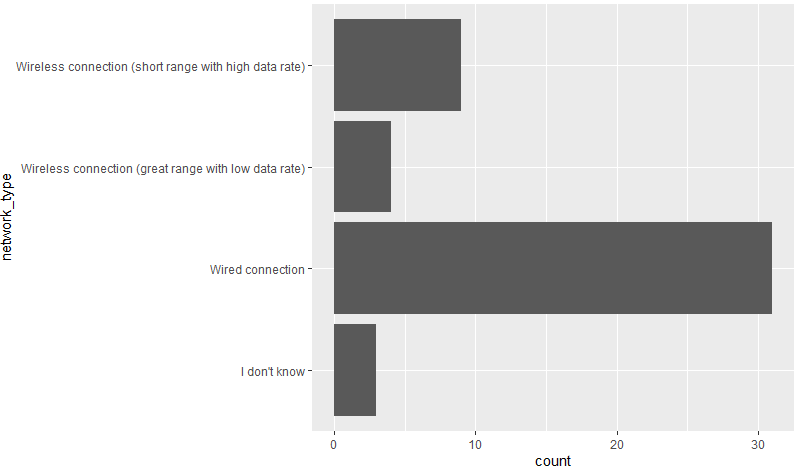
\includegraphics[width=12cm]{../img/network.png}
	
\end{figure}

The barplot shows that most people make use of a wired connection when they play games, where a few people use a wireless connection with either a great range (low data rate) or short range (high data rate). What was alos included in this survey was the question what system the interviewee uses to play video games, the most picked option was Windows/Microsoft. Which makes sense why the wired connection has been picked the most from this question, since wired connection is the most preferred connection type for PC gaming.

\begin{figure}[H]
	\centering
	\textbf{\caption{Question: Do you have a strong internet connection?}}
	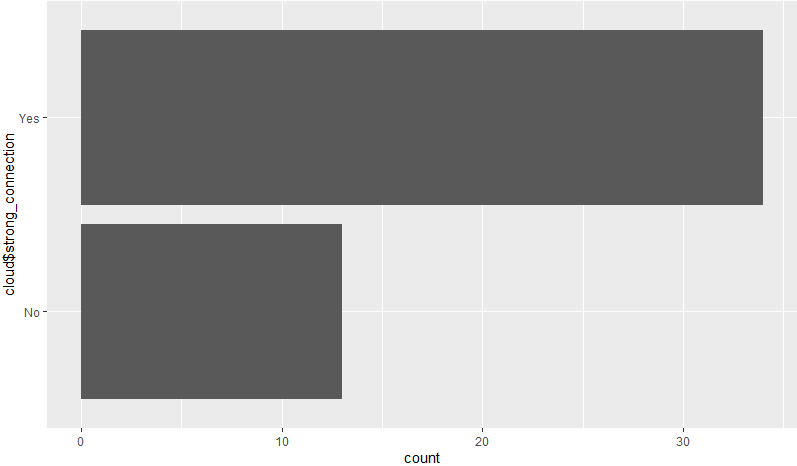
\includegraphics[width=12cm]{../img/connection.png}

\end{figure}

As shown in the chart above, most people claimed that they have a strong Internet connection, while a few people claimed that they do not have a strong Internet connection. We claimed from this that those who had chosen the option "No", that they use a wireless connection and the rest chose the option "Yes" because of a wired connection.

\begin{figure}[H]
	\centering
	\textbf{\caption{Question: When you play an online game, do you often have latency issues?}}
	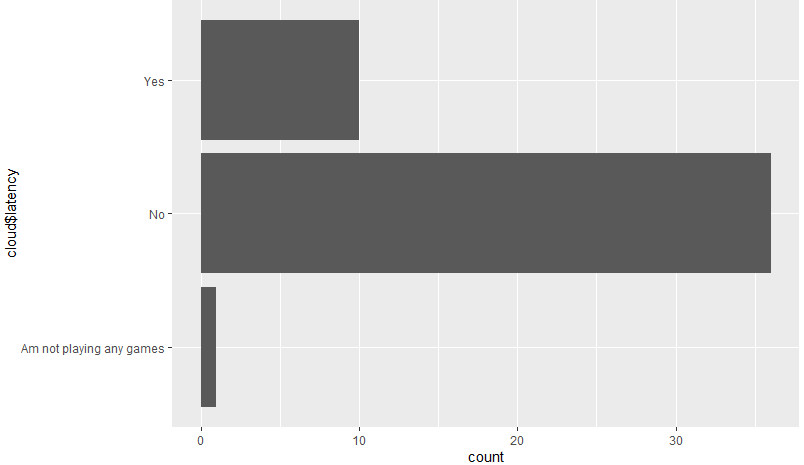
\includegraphics[width=12cm]{../img/latency.png}

\end{figure}

Most people said that they don't often experience latency/lag issues when they play an online game, but a few do experience latency. The people that answered "No" are most likely users of a wired internet connection, whereas the people that have said "Yes" are using a wireless connection.

\begin{figure}[H]
	\centering
	\textbf{\caption{Question: How interested are you in cloud gaming?}}
	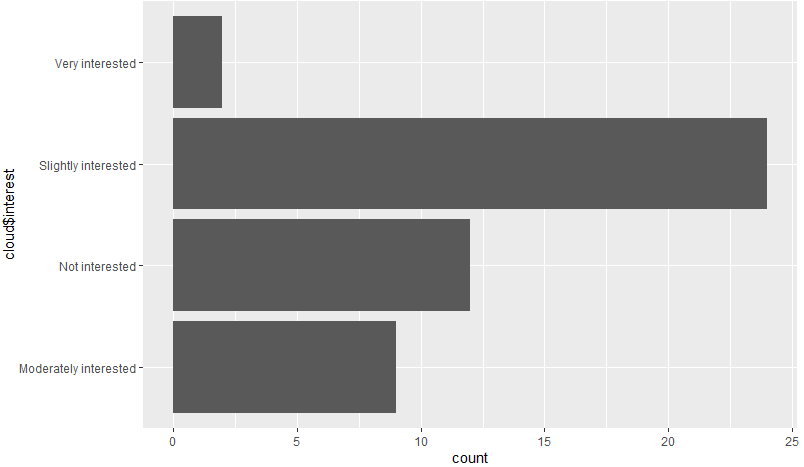
\includegraphics[width=12cm]{../img/interest.png}
	
\end{figure}

People had the choice to fill in how interested they are in cloud gaming. Most people have said that they are slightly interested in it. \\\textbf{From high to low:}\\\\
	Super interested\\
	Very interested\\
	Moderately interested\\
	Slightly interested\\
	Not interested\\\\
In the survey, we also had questions that were about the use of cloud gaming and what the respondents thought of it, such as: For cloud gaming you are attached to a monthly fee between 10 and 60 euros, that in cloud gaming you stream your games from a data center and not at home and that you require a strong and stable internet connection to make the best use of cloud gaming. Most interviewees had mixed thoughts about cloud gaming, which could have affected the question about the interest, having it mixed results. Half of all respondents gave it slight interest and a quarter chose to have no interest in it.

\begin{figure}[H]
	\centering
	\textbf{\caption{Question: Do you think cloud gaming has a future?}}
	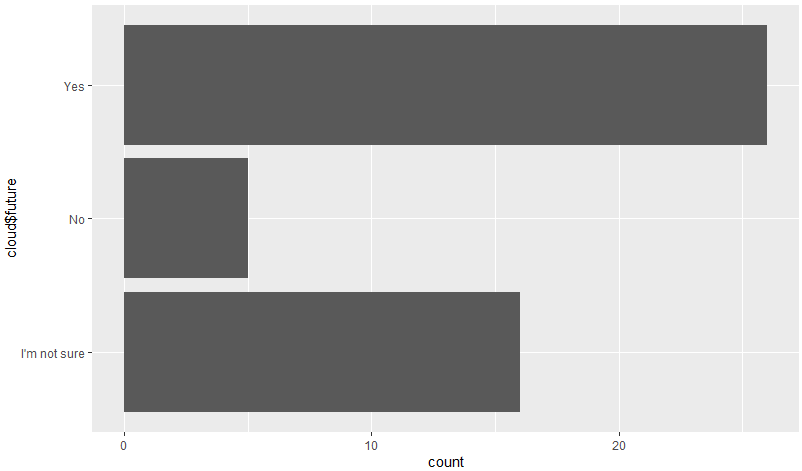
\includegraphics[width=12cm]{../img/future.png}

\end{figure}

For this question, respondents could answer whether cloud gaming has a future for video games. They could choose "Yes", "No" or "I'm not sure". Although there were mixed interests in cloud gaming, many believed that cloud gaming could have a future for video games, in which some did not believe in it, or were unsure about it

\begin{figure}[H]
	\centering
	\textbf{\caption{Question: How likely are you going to give cloud gaming a try?}}
	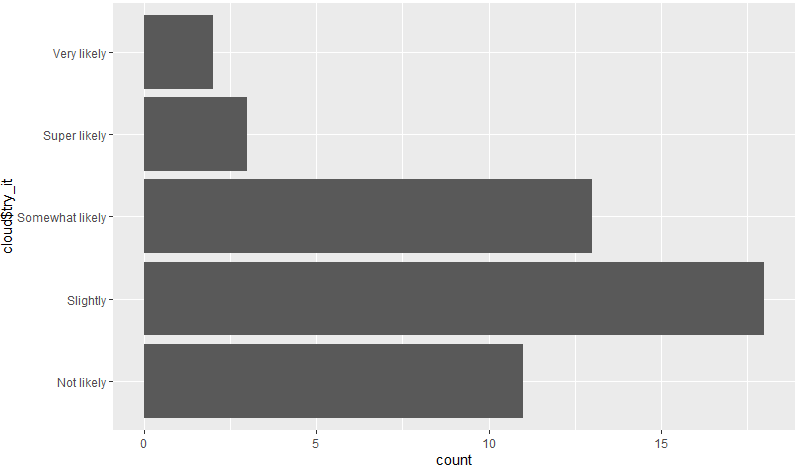
\includegraphics[width=12cm]{../img/try.png}
\end{figure}

Just like the question about how interested people were in cloud gaming, for this question people had the choice to fill in how likely they want to give cloud gaming a try. \\\textbf{From high to low:}\\\\
	Super likely\\
	Very likely\\
	Somewhat likely\\
	Slightly\\
	Not likely\\
	
This question was considered redundant by some interviewees. This could be true because the question about interest in cloud gaming was quite similar, only our thinking on this question was different. We saw this question as literally "Are you ever going to try cloud gaming?", but was changed to "How likely is it that you will try cloud gaming?", and most saw this as an unnecessary question because they had previously indicated whether they were interested in cloud gaming. In which the most frequently chosen option was "Slightly", as with the question about interest.
\\
\subsection{Research methods from articles}

We have come across a number of research articles related to cloud gaming, latency, and latency occurring in cloud gaming. Many articles used methods where they let people play in a cloud gaming environment and add an additional level of latency, to find out how people performed with the game that they were playing. 
\\\\
In the year 2020, \textcite{desveaux2020effects} performed a research about the effects of latency in commercial cloud gaming services. According to their Background and Related Work \parencite[Chapter 2.3, Page 17]{desveaux2020effects} increased latency generally has a negative impace on both player performance and Quality of Experience, whereby they wanted to conduct a similar experiment with it, by letting someone play Assassin's Creed Odyssey via different cloud gaming services with increased latency \parencite[Chapter 3, Page 18]{desveaux2020effects}.\\
After the experiment, \citeauthor{desveaux2020effects} collected the data into two separate types, subjective and objective data. For the subjective data \parencite[Chapter 4.2.2, Page 36]{desveaux2020effects}, the participants were asked to rate the graphics quality, responiveness of the controls and their willingness to continue playing under a certain added latency value.
\begin{figure}[H]
	\centering
	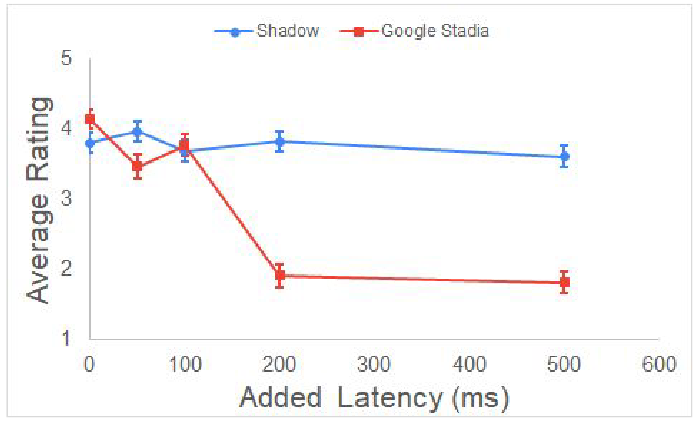
\includegraphics[width=12cm]{../img/fig13.png}
	\caption{Average Rating vs Added Latency for Graphics Quality}
	\parencite[Chapter 4.2.2, Page 36, Figure 13]{desveaux2020effects}
\end{figure}
\begin{figure}[H]
	\centering
	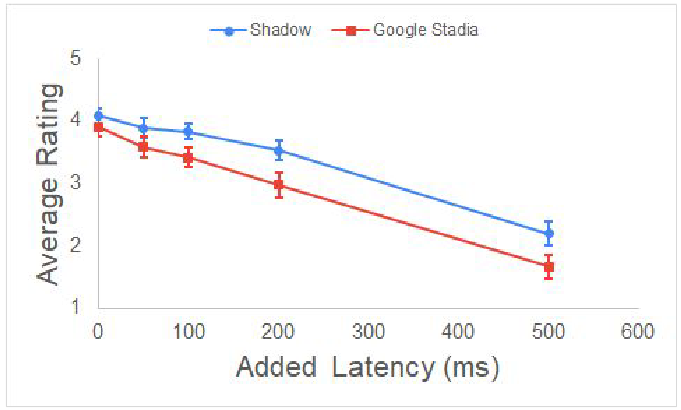
\includegraphics[width=12cm]{../img/fig14.png}
	\caption{Average Rating vs Added Latency for Responsiveness}
	\parencite[Chapter 4.2.2, Page 37, Figure 14]{desveaux2020effects}
\end{figure}
\begin{figure}[H]
	\centering
	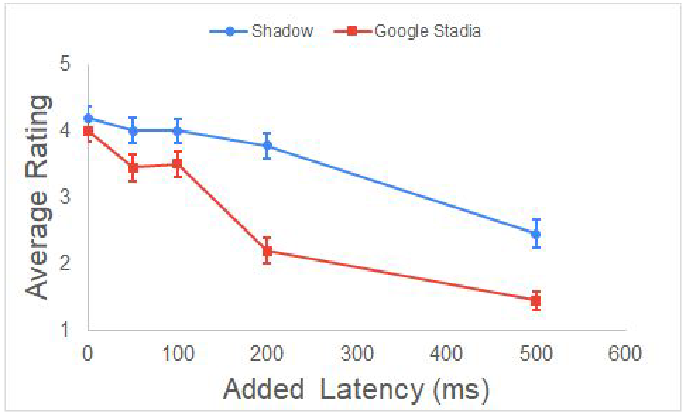
\includegraphics[width=12cm]{../img/fig15.png}
	\caption{Average Rating vs Added Latency for Willingness to play again}
	\parencite[Chapter 4.2.2, Page 37, Figure 15]{desveaux2020effects}
\end{figure}
The objective data \parencite[Chapter 4.2.3, Page 39]{desveaux2020effects} included the number of enemy kills as well as the number of times the participants were hit by enemy attacks.
\begin{figure}[H]
	\centering
	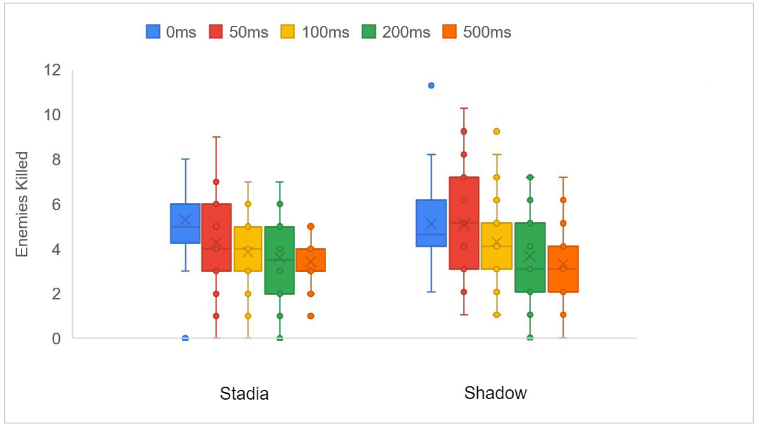
\includegraphics[width=12cm]{../img/fig16.png}
	\caption{Average Number of Enemies Killed for Various Added Latencies}
	In both services, the number of kills went downward as latency increased.\\
	\parencite[Chapter 4.2.3, Page 40, Figure 16]{desveaux2020effects}
\end{figure}
\begin{figure}[H]
	\centering
	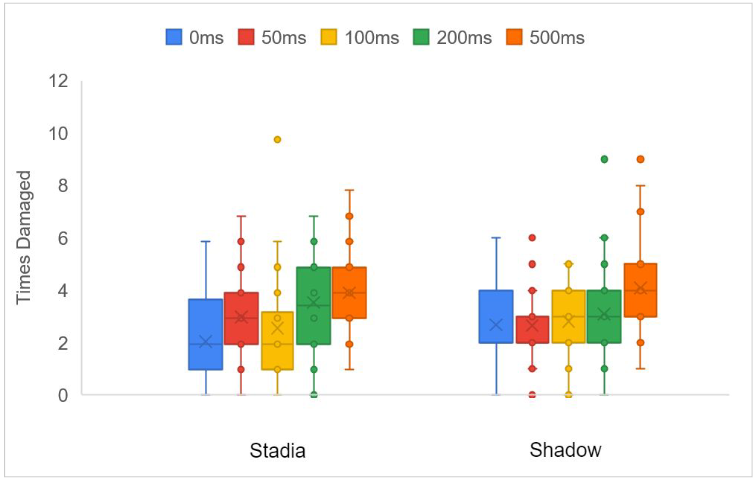
\includegraphics[width=12cm]{../img/fig17.png}
	\caption{Average Number of Times Damaged for Various Different Added Latencies}
	\parencite[Chapter 4.2.3, Page 40, Figure 17]{desveaux2020effects}
\end{figure}
\begin{figure}[H]
	\centering
	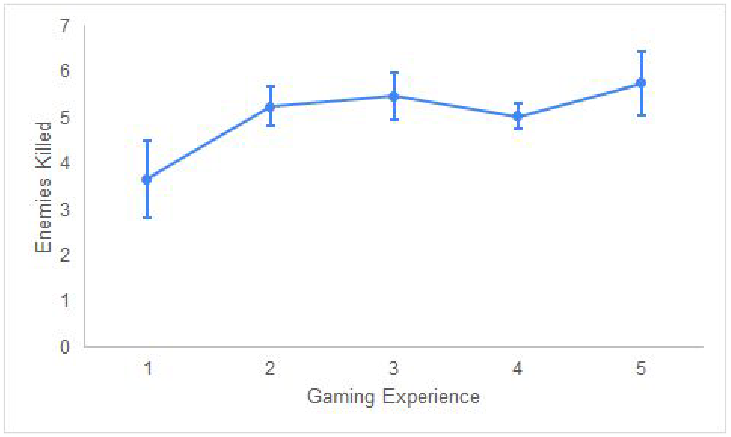
\includegraphics[width=12cm]{../img/fig18.png}
	\caption{Average Enemies Killed by Self Rated Gaming Experience}
	Number of kills went slightly upward depending on the gaming experience.\\
	\parencite[Chapter 4.2.3, Page 41, Figure 18]{desveaux2020effects}
\end{figure}
\begin{figure}[H]
	\centering
	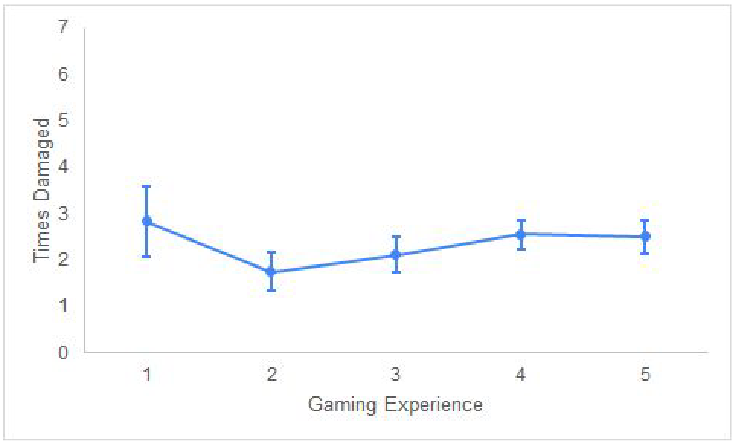
\includegraphics[width=12cm]{../img/fig19.png}
	\caption{Average Times Damaged by Self Rated Gaming Experience}
	\parencite[Chapter 4.2.3, Page 41, Figure 19]{desveaux2020effects}
\end{figure}
\newpage
\textcite{claypool2014effects} did perform a somewhat similar experiment where people play the game Crazy Taxi and Neverball on the cloud gaming services OnLive and GamingAnywhere \parencite[Chapter 3]{claypool2014effects}. In the game Crazy Taxi the player needs to earn points by driving a cab and transport as many customers to their destinations as quick as possible. Extra points can be earned by performing stunts with the cab \parencite[Chapter 3.A]{claypool2014effects}. In Neverball the player controls a stage level with a marble in it, the player needs to move the ball to its destination as fast as possible by tilting the stage with the arrow keys \parencite[Chapter 3.A]{claypool2014effects}. This experiment was done on older cloud gaming services.
\begin{figure}[H]
	\centering
	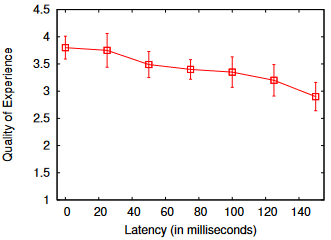
\includegraphics[width=12cm]{../img/fig20.png}
	\caption{QoE for Crazy Taxi on OnLive versus Latency}
	\parencite[Chapter 4, Figure 4]{claypool2014effects}
\end{figure}
\begin{figure}[H]
	\centering
	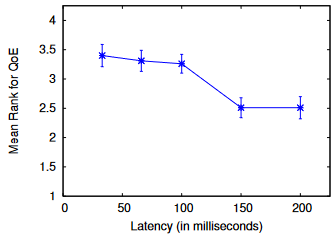
\includegraphics[width=12cm]{../img/fig21.png}
	\caption{QoE for Neverball on GamingAnywhere versus Latency}
	\parencite[Chapter 4, Figure 5]{claypool2014effects}
\end{figure}
\begin{figure}[H]
	\centering
	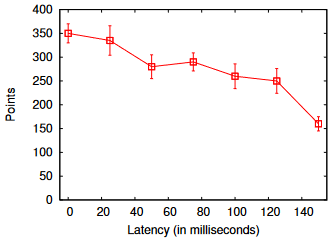
\includegraphics[width=12cm]{../img/fig22.png}
	\caption{User Points for Crazy Taxi on OnLive versus Latency}
	\parencite[Chapter 4, Figure 6]{claypool2014effects}
\end{figure}
\begin{figure}[H]
	\centering
	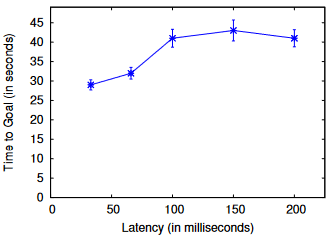
\includegraphics[width=12cm]{../img/fig23.png}
	\caption{User Times for Neverball on GamingAnywhere versus Latency}
	\parencite[Chapter 4, Figure 7]{claypool2014effects}
\end{figure}
\begin{figure}[H]
	\centering
	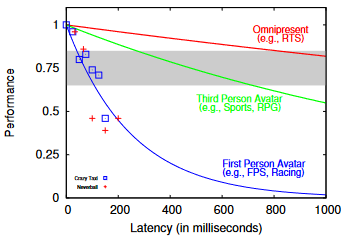
\includegraphics[width=12cm]{../img/fig24.png}
	\caption{User Performance versus Latency for Classes of Games}
	\parencite[Chapter 4, Figure 8]{claypool2014effects}
\end{figure}
\textcite{anouna2014network} also performed an experiment with the game Neverball that was using the cloud gaming service GamingAnywhere and used Dummynet to control the latency between the client and server \parencite[Chapter 3.2, Page 6]{anouna2014network}. One level was chosen for this experiment to measure the players' performances by the time it took them to complete the level \parencite[Chapter 4.1, Page 15]{anouna2014network}.
\begin{figure}[H]
	\centering
	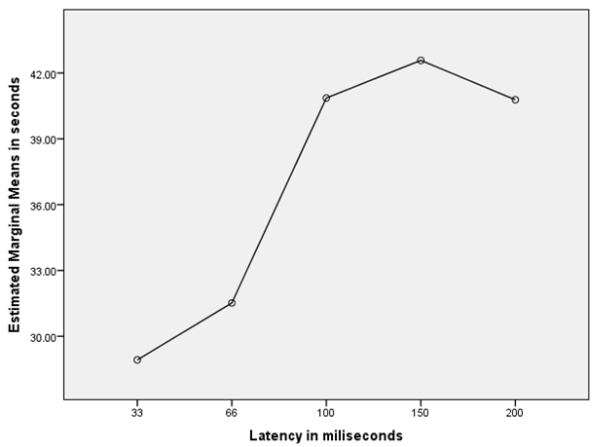
\includegraphics[width=12cm]{../img/fig25.png}
	\caption{A graph of the average time to complete at each latency}
	\parencite[Chapter 4.1, Page 15, Figure 4.1]{claypool2014effects}
\end{figure} 
\section{Discussion}

\subsection{Our conclusion}
From what we picked up from our research form, and from the research articles we found, latency plays a very important role in the widespread adaptation of cloud gaming. Found from \textit{figure 7, 8, 18, chapter 3.2}, we have found that the higher the latency plays up with a cloud gaming service, that the performance quality can go down with a marked difference to little latency. Not only does increased latency cause performance to go down, but also the client's gaming experience, shown in \textit{figure 9, 14, 15, 16, 17, chapter 3.2}. While most from the survey form claimed to have a strong internet connection with little or no latency issues, most had little or no interest in the concept of cloud gaming. However, we do not think this is due to latency, given that everyone from the survey were using a gaming computer, or home console, they would therefore not make a quick switch to cloud gaming if they already have hardware to play on. Still, most felt that cloud gaming has potential in the future, which we also found from \parencite[Chapter VI]{7536162}.\\

\subsection{What we can improve}
Many questions in our survey contained checkboxes where you could make more than one choice, most of the data became attributes with multiple values, which made it very difficult to visualize the data. Something else that was not very smart to include in our survey was the option to leave an open answer, which also led to difficult visualization. For the next survey we may create, we will leave out the open-answer option and make more use of closed questions or multiple-choice answers (one answer possible), to avoid attributes with multiple values and difficult visualisations. 

this is cited \cite{claypool2014effects}
\printbibliography[title=References]



\end{document}
	
\printbibliography[title=References]
	
	
	
	
	
	
	
	
	
	
	
	
	
	
	
	
	
	
	
	
	
	
  
